\documentclass[12pt,aspectratio=43]{beamer}
\usepackage{tikz}
\usetheme{Madrid}
\setbeamertemplate{navigation symbols}{}
\title{Geometric uncertainty: experiments and bounds}
\subtitle{Generated interaction study}
\author{Research group}
\date{}
\year=2026\month=11\day=5
\newcommand{\fuzzlayerA}[1]{\textbf{#1}}
\newcommand{\fuzzlayerB}[1]{\fuzzlayerA{#1}}
\newcommand{\fuzzlayerC}[1]{\fuzzlayerB{#1}}
\newcommand{\fuzzterm}[1]{\fuzzlayerC{#1}}
\newcommand{\fuzzpair}[2]{\fuzzterm{#1}: #2}
\newcommand{\fuzzunit}{Hz}
\let\fuzzoriginalunit\fuzzunit
\newcommand{\fuzzcoefficient}{2}
\newcommand{\fuzzscale}[2][\fuzzcoefficient]{#1\,#2}
\definecolor{fuzzpaint}{RGB}{255,0,255}
\definecolor{fuzzsecond}{RGB}{18,137,67}
\tikzset{fuzzvertex/.style={draw,rounded corners=1pt,fill=blue!10,inner sep=1pt,minimum width=.35cm,minimum height=.25cm}}
\begin{document}
\section{Geometric uncertainty}
\begin{frame}[t,shrink=5]{Geometric uncertainty}{Composed dependencies}
\fuzzpair{Experiment}{Timing: 12\fuzzunit; estimate $\fuzzscale{x}+\fuzzscale[2]{y}$.}\par
{\renewcommand{\fuzzunit}{cycles}\let\fuzzterm\textrm\fuzzpair{LocalScope}{Timing: 7\fuzzunit.}\par}
\fuzzpair{RestoredScope}{Timing: 11\fuzzunit.}\par
\visible<1-2>{\begin{columns}[onlytextwidth,c]
\begin{column}{0.38\textwidth}
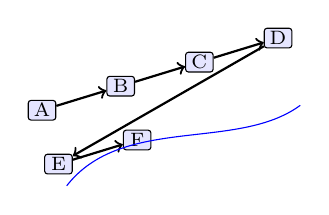
\begin{tikzpicture}[font=\scriptsize]
\begin{scope}[scale=1.1,rotate=17]


\node[fuzzvertex] (g3n0) at (0.000,0) {A};
\node[fuzzvertex] (g3n1) at (0.950,0) {B};
\node[fuzzvertex] (g3n2) at (1.900,0) {C};
\node[fuzzvertex] (g3n3) at (2.850,0) {D};
\node[fuzzvertex] (g3n4) at (0.000,-0.65) {E};
\node[fuzzvertex] (g3n5) at (0.950,-0.65) {F};
\begin{scope}[xshift=.5pt,yshift=-.5pt]
\draw<1->[->,thick] (g3n0) -- (g3n1);
\draw<1->[->,thick] (g3n1) -- (g3n2);
\draw<1->[->,thick] (g3n2) -- (g3n3);
\draw<1->[->,thick] (g3n3) -- (g3n4);
\draw<1->[->,thick] (g3n4) -- (g3n5);
\draw[blue] (0,-.9) .. controls (0.855,-.3) and (1.995,-1.1) .. (2.850,-.8);
\end{scope}
\end{scope}
\end{tikzpicture}
\end{column}
\begin{column}{0.58\textwidth}
\begin{description}
\item[Stage 1] \textit{A narrow column} can change line breaking even when the underlying expression is unchanged. A local update can change the measurements used by several neighboring components. The estimate is $\frac{a+b}{1+c}$.
\item[Stage 2] \[\begin{pmatrix}a&b\\c&d\end{pmatrix}\begin{pmatrix}x\\y\end{pmatrix}\]
\item[Stage 3] \begin{tabular}{lrr}Method&Cost&Error\\\hline
Local0&12&29\\
Fresh1&0&15\\
Global2&3&1\\
Local3&10&0\\
\end{tabular}
\end{description}
\end{column}
\end{columns}
\par
\begin{columns}[onlytextwidth,T]
\begin{column}{0.38\textwidth}
\visible<2->{\textrm{A local update} can change the measurements used by several neighboring components.  The estimate is $x_i+x_{i+1}$.}
\end{column}
\begin{column}{0.58\textwidth}
\begin{alertblock}{Incremental analysis}
\begin{description}
\item<1->[Stage 1] \textrm{A local update} can change the measurements used by several neighboring components.  The estimate is $\frac{a+b}{1+c}$.
\item<2->[Stage 2] \[\begin{aligned}a+b&=c\\ d-e&=f\end{aligned}\]
\end{description}
\end{alertblock}
\end{column}
\end{columns}}
\par 
\begin{tikzpicture}[font=\scriptsize]
\fill<2-3>[fuzzpaint] (0,0) rectangle (.8,.3);
\fill<3->[fuzzsecond] (1,0) rectangle (1.8,.3);
\node[anchor=west] at (2,0.15) {Witness};
\end{tikzpicture}
\only<4>{}
\end{frame}
\renewcommand{\fuzzunit}{us}
\renewcommand{\fuzzcoefficient}{2}
\renewcommand{\fuzzterm}[1]{{\textit{#1}}}
\section{Cache invalidation}
\begin{frame}[t]{Constraint propagation}
\fuzzpair{MacroStageB}{Timing: 12\fuzzunit, retained: 9\fuzzoriginalunit.}\par
{\renewcommand{\fuzzunit}{local}\fuzzpair{FrameLocal}{Timing: 5\fuzzunit.}\par}
\fuzzpair{FrameRestored}{Timing: 8\fuzzunit; estimate $\fuzzscale{x}$.}\par
\begin{columns}[T]\begin{column}{.46\textwidth}We compare the proposed solution with a reference computed from the complete input.\end{column}\begin{column}{.46\textwidth}\begin{itemize}\item Input state\item Updated state\end{itemize}\end{column}\end{columns}
\end{frame}
\renewcommand{\fuzzunit}{s}
\renewcommand{\fuzzcoefficient}{3}
\renewcommand{\fuzzterm}[1]{{\textrm{#1}}}
\section{Geometric uncertainty}
\begin{frame}[t]{Incremental analysis}
\fuzzpair{MacroStageC}{Timing: 12\fuzzunit, retained: 9\fuzzoriginalunit.}\par
{\renewcommand{\fuzzunit}{local}\fuzzpair{FrameLocal}{Timing: 5\fuzzunit.}\par}
\fuzzpair{FrameRestored}{Timing: 8\fuzzunit; estimate $\fuzzscale{x}$.}\par
\begin{block}{Follow-up}\fuzzterm{A revised value} depends on the preceding frame.\end{block}
\[r_{k+1}=r_k-\alpha d_k\]
\end{frame}
\renewcommand{\fuzzunit}{min}
\renewcommand{\fuzzcoefficient}{4}
\renewcommand{\fuzzterm}[1]{{\textbf{#1}}}
\section{Message passing}
\begin{frame}[t]{Constraint propagation}
\fuzzpair{MacroStageD}{Timing: 12\fuzzunit, retained: 9\fuzzoriginalunit.}\par
{\renewcommand{\fuzzunit}{local}\fuzzpair{FrameLocal}{Timing: 5\fuzzunit.}\par}
\fuzzpair{FrameRestored}{Timing: 8\fuzzunit; estimate $\fuzzscale{x}$.}\par
\begin{columns}[T]\begin{column}{.46\textwidth}Intermediate results carry both a numerical estimate and an explicit dependency set.\end{column}\begin{column}{.46\textwidth}\begin{itemize}\item Input state\item Updated state\end{itemize}\end{column}\end{columns}
\end{frame}
\end{document}
